\documentclass{beamer}
\usetheme{manhattan}  % Now it's a beamer presentation with the Manhattan College theme!

\usepackage{url}
\usepackage{graphicx}
\usepackage{../salgorithm}
\usepackage{verbatim}
\usepackage{amsthm, amsfonts, amsmath, amssymb, amsxtra}

\newcommand{\NP}{\ensuremath{\mathcal{NP}}}
% Make a new command that will make a new subsection and a frame with the same title
\newcommand{\fst}[2]{\subsection{#1}\frame{\frametitle{#1} #2}}

\title{Using Cell Phone Keyboards is \NP\ Hard }
\author{Peter Boothe}
\date{2 June 2010\\
FUN With Algorithms}
\institute[Manhattan College]{
    \url{peter.boothe@manhattan.edu}\\
    Mathematics and Computer Science \\
    Manhattan College}

\begin{document}
\frame{\titlepage}

\section{Introduction}

\fst{So many letters \ldots}{
\begin{itemize}
    \item People want to use phones to send text messages
    \item English has 26 letters, and each letter cas a lower-case and capital form, and we should not forget numbers, puctuation, and whitespace characters.
    \item Other languages have even more!\footnote{Can you name a language with fewer letters than English?\\}
\end{itemize}
}

\fst{\ldots so few keys}{
\begin{tabular}{c p{2.5in}}
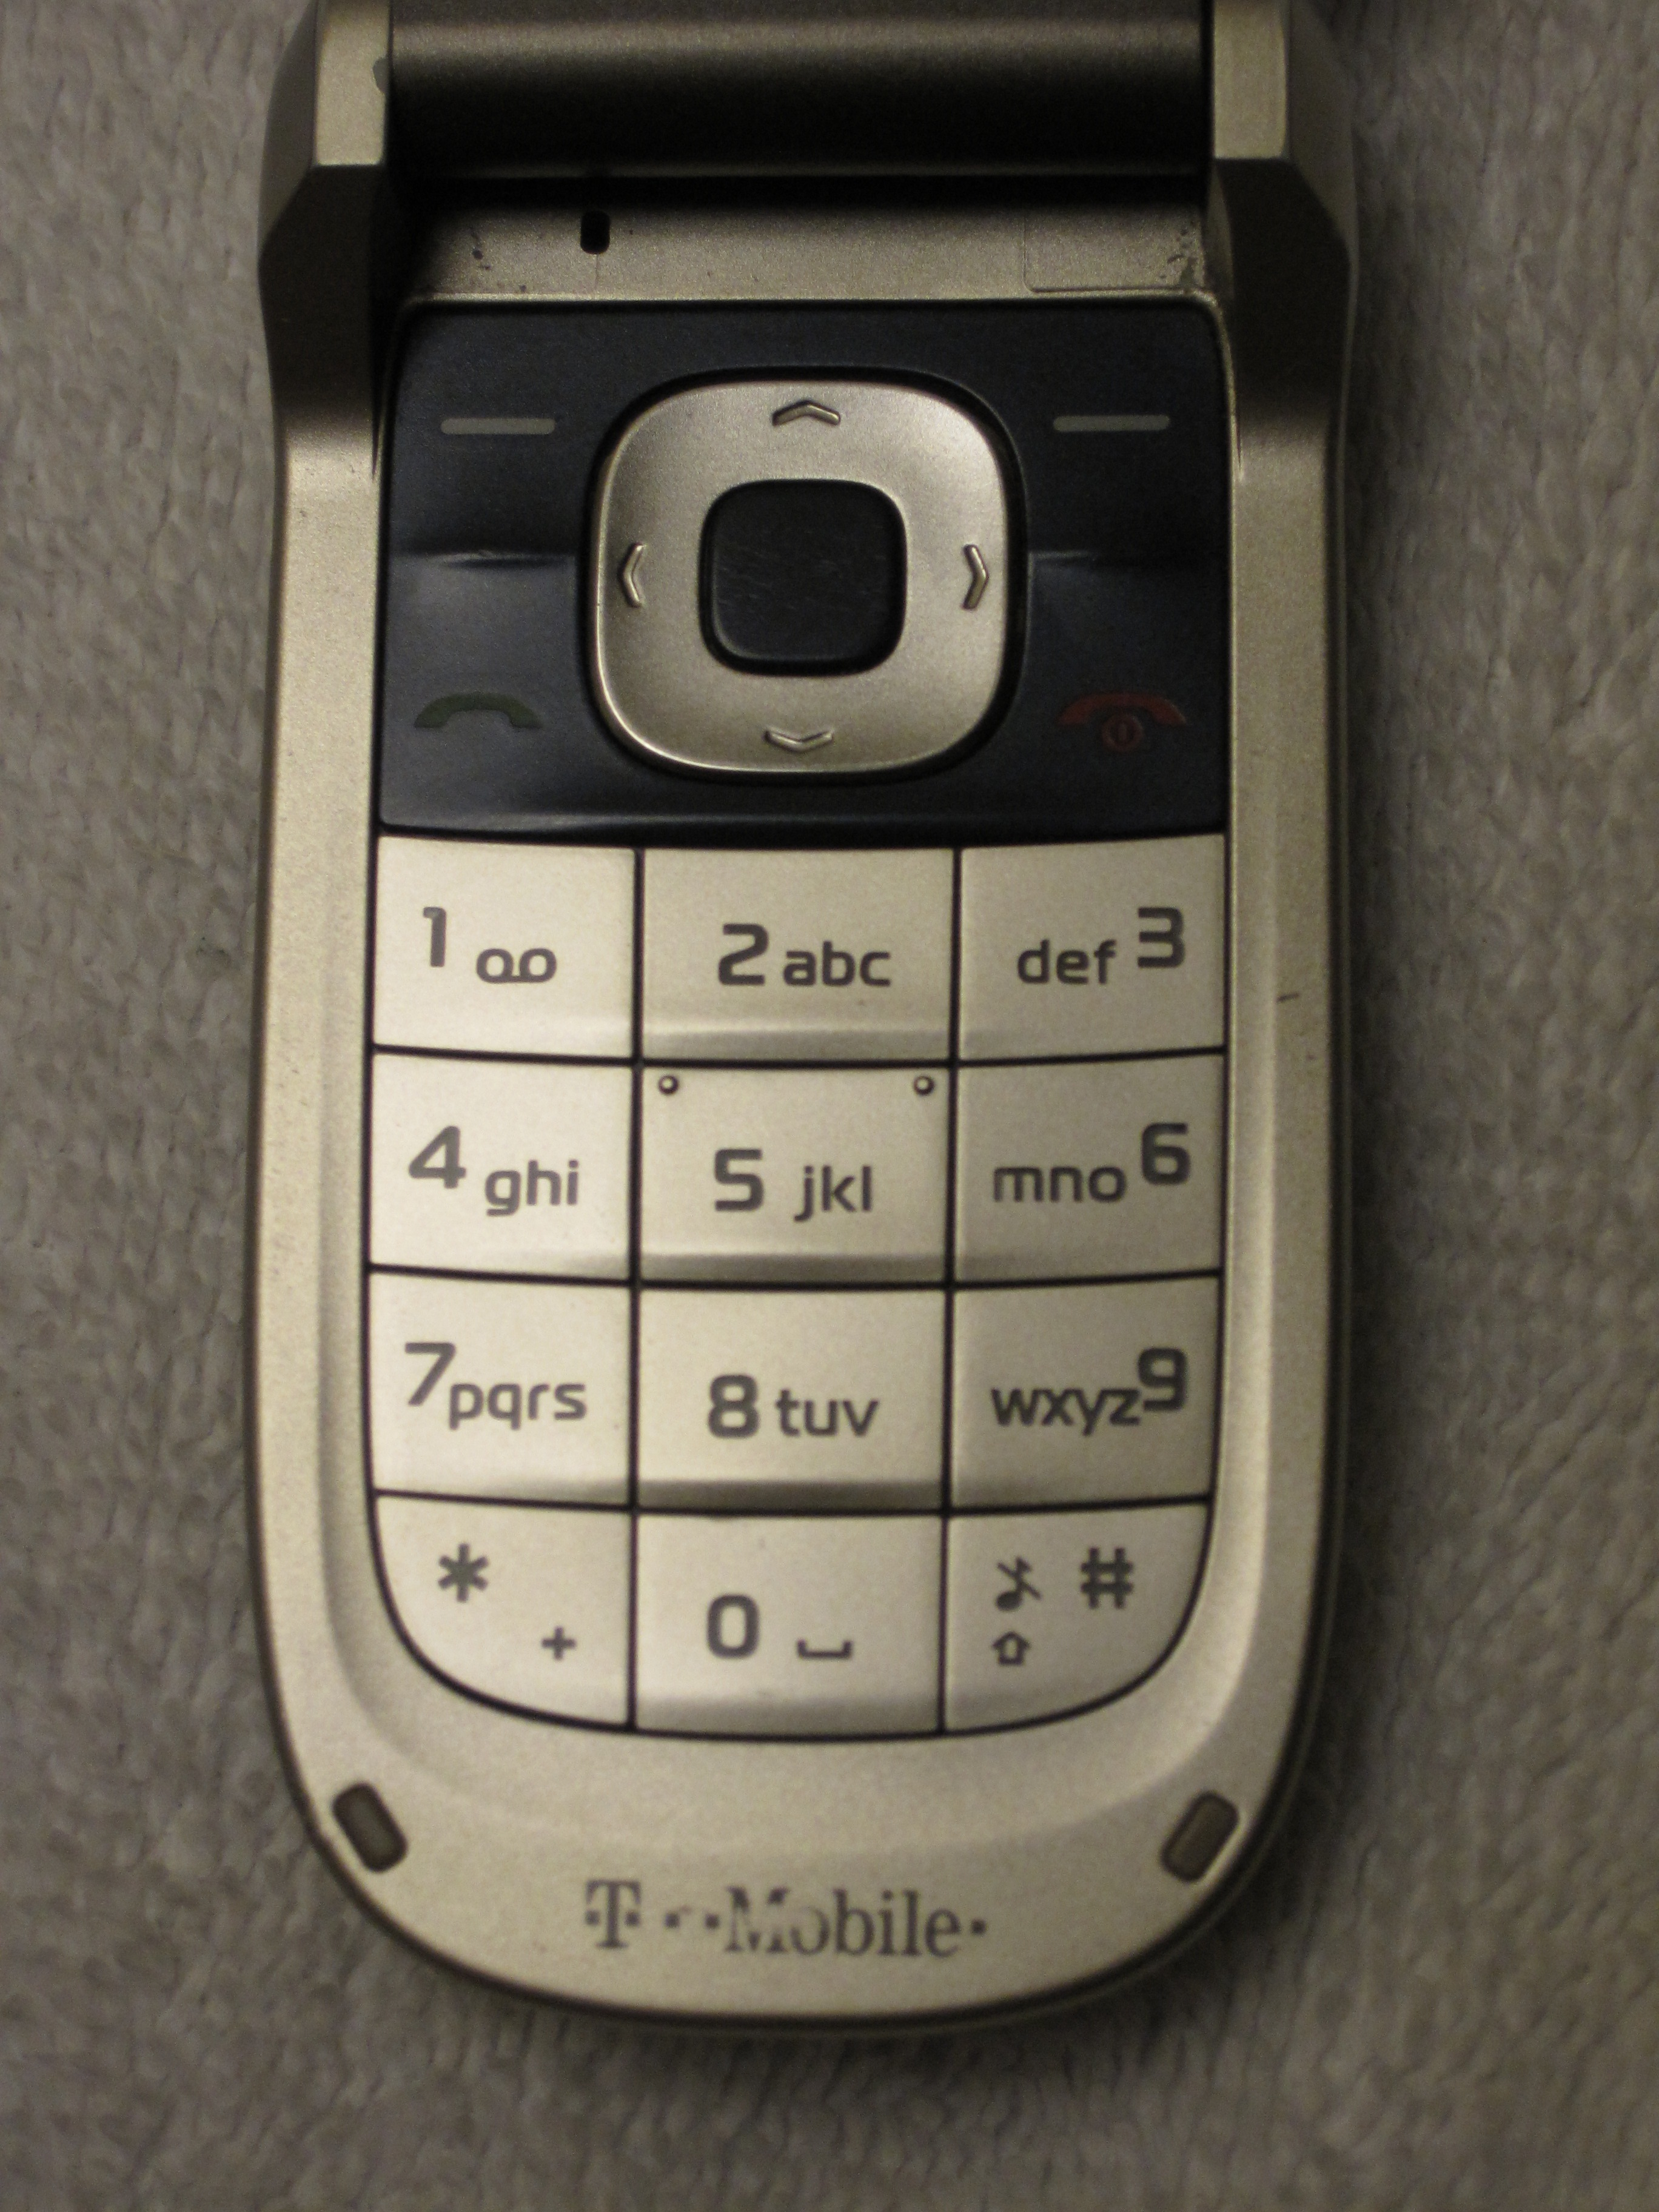
\includegraphics[width=1.5in]{../phonekeys.jpg} & 
\vspace{-2in}
\begin{itemize}
    \item A computer keyboard usually has more than 100 keys.
    \item A phone keyboard has, depending on the model, as few as 8 keys which may be used to input letters.
\end{itemize}
\end{tabular}
}

\fst{Two Input Methods}{
    The old default mapping of numbers to letter sequences:
\begin{center}
\begin{tabular}{l l l}
1 $\to$ [] & 2 $\to$ [a,b,c] & 3 $\to$ [d,e,f] \\
4 $\to$ [g,h,i] & 5 $\to$ [j,k,l] & 6 $\to$ [m,n,o] \\
7 $\to$ [p,q,r,s] & 8 $\to$ [t,u,v] & 9 $\to$ [w,x,y,z]
\end{tabular}
\end{center}

\vspace{.25in}
\begin{description}
    \item[Standard] Press the appropriate key until your letter appears.  e.g. Press 8 two times to get a `u'
    \item[T-9] Load a word-frequency dictionary for the language into the phone, and only require that people type one key for each character.  Display the most popular word with a given keypress sequence.
\end{description}
}

\fst{Our question}{
    Both of these input methods assume the old default mapping.  If we throw that assumption out, then, for each typing method: \\
\vspace{.5in}
\LARGE{\it What is the mapping of numbers to letters that minimizes the number of keypresses required to type a message?}
}

\fst{Our question, formalized}{
\begin{description}
\item[\sc Instance] A number of keys, $k$, an alphabet $A$, an input method $\mathrm{IN}: (word, partition) \to {\Bbb N}$, and a set of words and associated frequencies $W$.  
\item[\sc Question] What is the partition $P$ of $A$ into $k$ sequences which minimizes
$$\sum_{(w,f)\in W} f \times\mathrm{IN}(w,P)$$
?
\end{description}
}

\section{Standard Input Method}
\fst{The Standard Input Method}{
\begin{itemize}
    \item Press a key as many times as needed to made the desired letter appear
    e.g. ``fun'' is 3338866, requiring a total of 7 button presses
    \item Word-independent
    \item Easy to understand
    \item Inefficient  e.g. $7 \to [p,q,r,s]$ means you have to go through `q' to get to `r' or `s'
\end{itemize}
}
\fst{Greedy Algorithm}{
\begin{itemize}
    \item Sort the alphabet by letter frequency.
    \item Assign letters to keys in round-robin order.
    \item Proven optimal via an exchange argument (see paper)
    \item Rearranges the letters on the keys
    \item Possibly a very confusing layout
\end{itemize}
}
\fst{Legacy-Preserving Greedy Algorithm}{
\begin{itemize}
    \item Sort each key's letters by frequency.  Reorder the letters on each key in decreasing frequency order.
    \item Using the British National Corpus, this reduces button presses by 28.43\% 
    \item Less confusing than remapping the whole keyboard
    \item Just fixing the 7 key will save you $\sim$10\%
\end{itemize}
}
\fst{An Open Letter}{
Dear Cell Phone Manufacturers,\\
~\\
\hspace{.25in}Please change your keyboard layout to:\\
\begin{center}
\begin{tabular}{l l l}
1 $\to$ [] & 2 $\to$ [a,c,b] & 3 $\to$ [e,d,f] \\
4 $\to$ [i,g,h] & 5 $\to$ [l,k,j] & 6 $\to$ [o,n,m] \\
7 $\to$ [s,r,p,q] & 8 $\to$ [t,u,v] & 9 $\to$ [w,y,x,z]
\end{tabular}
\end{center}
\hspace{.25in}This new layout will require your customers to type 28\% fewer keystrokes when sending an SMS message, but will not break such famous numbers as 1-800-FLOWERS, 1-800-MARINES, or PA-6-5000.  Or at least fix the 7 key.
~\\
\hspace{3in}Sincerely,\\
\hspace{3in}Peter Boothe
}

\section{T-9 Input Method}
\fst{The T-9 Input Method}{
\begin{itemize}
    \item Per-word, not per-character
    \item One key per letter, display the most popular word with that key sequence e.g. `home' is 4663.
    \item In case of collision, cycle through all words with that key sequence in order of popularity using * e.g. `home', `good', `gone', `hood', `hoof', `hone', and `goof' are all 4663, so `goof' is 4663******
    \item Two words with the same sequence are {\bf t9onyms}
\end{itemize}
\begin{center}
    Can we minimize the expected number of * key presses?\\
or, equivalently,\\
    Can we minimize the expected number of t9onyms?
\end{center}
}

\fst{Minimizing T-9 is \NP-complete}{
\begin{itemize}
    \item We have sequences in the problem (the words in the dictionary)
    \item We have partitions in the problem (the assignment of letters to keys)
    \item Couldn't find a NPC problem with both, so invented one
    \item Proof is via reduction from {\sc UniquePathColoring}
\end{itemize}
}

\fst{{\sc UniquePathColoring}}{
\begin{description}
\item[\sc Instance] A graph $G = (V , E)$, a set of paths $P$, and a parameter $k$.
\item[\sc Question] Is there a $k$-coloring of $V$ such that every path in $P$ has a unique coloring?
\end{description}

Note that this problem meets our criteria of having sequences (the paths of $P$ which correspond eventually to the words in $W$) and partitions (the colors of the graph, which correspond eventually to the key assigned to each letter).  {\sc UniquePathColoring} is equivalent to asking if there is an assignment with no t9onyms.
}

\fst{{\sc UniquePathColoring} is \NP-Complete}{
Reduction from {\sc GraphColoring}.\\
~\\
Take the $G=(V,E)$ and $k$ from {\sc GraphColoring}, and construct $G'$.
\begin{eqnarray*}
G' = & ( & V \cup \{0, 1\}, \\
& & E \cup \{(1,1), (0,1), (0,0)\} \cup \{ (v,0)~\forall v \in V \}\\
& ) &
\end{eqnarray*}
}

\frame{
\frametitle{{\sc UniquePathColoring} is \NP-Complete (2)}

Next, uniquely number the edges in $E$.
Construct $P$ by making paths $p_i$ for each edge $(u,v)$ in $E$.
\begin{eqnarray*}
p_i = & \{ & [ u, 0, \mathrm{b}_1(i), \mathrm{b}_2(i), \ldots \mathrm{b}_{\lceil \log_2 i \rceil}(i) ],\\
      &    & [ v, 0, \mathrm{b}_1(i), \mathrm{b}_2(i), \ldots \mathrm{b}_{\lceil \log_2 i \rceil}(i) ],\\
      &  \} & 
\end{eqnarray*}
where $\mathrm{b}_j(i)$ is the $j$th binary digit of $i$.

$$P = \bigcup_{1 \le i \le |E|} p_i$$
}

\frame{
\frametitle{{\sc UniquePathColoring} is \NP-Complete (3)}
    Does there exist a {\sc UniquePathColoring} of $G'$ with paths $P$ using no
more than $k$ colors?  If so, then the colors assigned to the vertices in $V$
form a $k$-coloring of $G$.\\
~\\
    Does there exist a $k$-coloring of $G$?  If so, we can construct a {\sc UniquePathColoring} of $G'$ and $P$ using $k$ colors --- simply choose two distinct colors for the new vertices 0 and 1.\\
~\\
$\therefore$ {\sc UniquePathColoring} is \NP-complete
}

\fst{{\sc Minimum-T9onyms} is \NP-complete}{
    The decision problem {\sc Minimum-T9onyms}:
\begin{description}
    \item[\sc Instance] Alphabet $A$, set of words and associated frequencies $W$, number of keys $k$, number $t$.
    \item[\sc Question] Is there a partition of $A$ into $k$ sets such that
\[t \ge \sum_{(w,f)\in W} f\times(\mathrm{len}(w) + \mathrm{order}(w,P,W,f))~~?\]
\end{description}

Note that this exactly conforms to our problem specification from the beginning.
}

\frame{
\frametitle{{\sc Minimum-T9onyms} is \NP-complete (2)}
If we require that there be no t9onyms, then this simplifies to 
\[t \ge \sum_{(w,f)\in W} f\times\mathrm{len}(w)\]
or simply a requirement that order$()$ be zero for all words in $W$.\\
}

\frame{
\frametitle{{\sc Minimum-T9onyms} is \NP-complete (3)}
The reduction from {\sc UniquePathColoring}\ldots\\
\vspace{.25in}
\begin{tabular}{p{2in} | p{1.97in}}
{\sc UniquePathColoring} & {\sc Minimum-T9onyms} \\
\\
{\sc Instance}~~Graph $G=(V,E)$, paths $P$, and $k$ colors &
{\sc Instance}~~Alphabet $V$, words $P$ all with frequency 1, number of keys $k$, and $t = \sum_{p\in P} \mathrm{len}(p)$ \\
~\\
{\sc Question}~~Does there exist a $k$-coloring of $V$ such that every path $p\in P$ has a unique coloring? &
{\sc Question}~~Does there exist a $k$-partition of $V$ such that every word $p\in P$ has order$()$ zero? 
\end{tabular}
\qed
}

\section{Numerical Results for T-9}
\fst{Baseline}{Our baseline comparison was the number of keystrokes required to enter the entire British National Corpus using T-9 with the standard layout.

\vspace{.25in}
T-9, with the default layout, requires 443,374,079 keypresses to enter the entire BNC.}

\fst{Enumerating All Alphabetic Partitions}{
If we restrict ourselves to only the partitions which keep the letters in alphabetic order, then we can enumerate all $\binom{25}{7}$ partitions and test them over the course of a few days on a modern computer.

\vspace{.25in}
We find that the best partition is
\[\{\{ab\}, \{cde\}, \{fghij\}, \{klm\}, \{nop\}, \{qrs\}, \{t\}, \{uvwxyz\}\} \] This partition requires 442,717,436 keypresses, a savings of 656,643 keypresses, or $0.14\%$. 
}
\fst{Genetic Algorithm Results}{
A very simple genetic/stochastic algorithm was run for a few days.  The best solution found was 
\[\{\{be\},\{cdl\},\{hs\},\{mxz\},\{afgy\},\{jot\},\{npuv\},\{ikqrw\}\}\]
This required 441,612,049 keypresses, a savings of 1,762,030 keypresses, or $0.40\%$.
}

\section{Summary}
\fst{Future Work}{
\begin{itemize}
    \item Predictive T-9
    \item Other input methods
    \item When T-9 gets a misspelled word, it is very bad and confusing.  Can we minimize not just t9onyms, but also the number of words that have a cell-phone Levenshtein distance of 1? of 2? of $k$?
    \item We completely ignored the pauses that the standard method requires when typing two letter in a row which involve the same key
    \item Completely solving the particular case of T-9 with the English language and an 8-key keyboard
\end{itemize}
}
\fst{Take-away Messages}{
\begin{itemize}
    \item Cell phone keyboards can provide algorithmic fun
    \item The standard input method can be optimized with the greedy algorithm
    \item The T-9 input method is NP-Complete to optimize
    \item The existing keyboard seems alright for T-9, but can be improved by 28\% for the standard input method without breaking legacy advertising
    \item Cell phone keyboards are not just hard to use, they can also be \NP-hard to use
\end{itemize}
}

\fst{Thanks!}{\begin{center}{\Huge\bf Questions?}\end{center}}

\end{document}
